\documentclass[a4paper, 12pt]{article}
\usepackage[left=1.5cm, right=1.5cm, top=1.5cm, bottom=2.5cm]{geometry}
\usepackage[utf8]{inputenc}
\usepackage[russian]{babel}
\usepackage{verbatim}
\usepackage{graphicx}
\usepackage{listingsutf8}
\usepackage{color}
\usepackage{ulem}
\usepackage{amsmath}
\usepackage{array}
\usepackage{amssymb, latexsym, amsmath, textcomp}
\usepackage{indentfirst}
\usepackage{cmap}
\usepackage{graphics}
\usepackage{listings}
\usepackage{enumerate}

\lstset{
basicstyle=\footnotesize,
breaklines=true,
numbers=left,
extendedchars=\true,
numbersep=7pt,
caption=\lstname,
frame=single,
inputencoding=utf8,
showstringspaces=\false
}

\newenvironment{enumerate*}%
  {\begin{enumerate}%
    \setlength{\itemsep}{1pt}%
    \setlength{\parskip}{1pt}}%
  {\end{enumerate}}
\newenvironment{itemize*}%
  {\begin{itemize}%
    \setlength{\itemsep}{1pt}%
    \setlength{\parskip}{1pt}}%
  {\end{itemize}}

%------------------------------------------------------------------------------------------------------------------------------
%------------------------------------------------------------------------------------------------------------------------------
\begin{document}

\begin{titlepage}
\begin{center}
{Санкт-Петербургский национальный исследовательский университет информационных технологий, механики и оптики}

Кафедра вычислительной техники
\end{center}
\vspace{50mm}
\begin{center}
\begin{tabular}{c}
\Huge{\textbf{Отчёт}}\\
\Large{\textbf{по лабораторной работе №1}}\\
\Large{\textbf{дисциплины <<Программирование интернет-приложений>>}}\\
\Large{\textbf{Вариант №305}}\\[2mm]
\end{tabular}
\end{center}
\vspace{85mm}
\begin{flushright}
\begin{tabular}{l}
Выполнили:\\
студенты гр. P3211\\
Ефремов Р.В.,\\
Синицкий Д.П.\\
Преподаватели:\\
Цопа Е.А.\\
Письмак А.Е.\\
\\
\end{tabular}
\end{flushright}
\vspace{15mm}
\begin{center}
Санкт-Петербург - 2017 г.
\end{center}
\end{titlepage}
\newpage

\section{Текст задания}

Разработать PHP-скрипт, определяющий попадание точки на координатной плоскости в заданную область, и создать HTML-страницу, которая формирует данные для отправки их на обработку этому скрипту.

Параметр R и координаты точки должны передаваться скрипту посредством HTTP-запроса. Скрипт должен выполнять валидацию данных и возвращать HTML-страницу с таблицей, содержащей полученные параметры и результат вычислений - факт попадания или непопадания точки в область.

Кроме того, ответ должен содержать данные о текущем времени и времени работы скрипта.

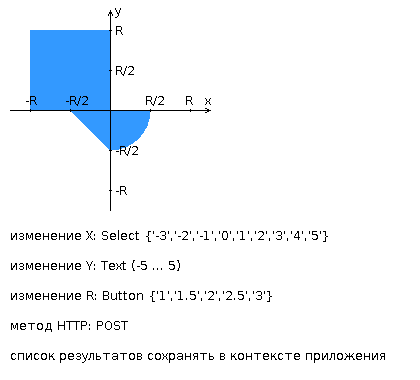
\includegraphics[scale=0.6]{img/areas.png}

\paragraph{Разработанная HTML-страница должна удовлетворять следующим требованиям:}

\begin{itemize*}
\item Для расположения текстовых и графических элементов необходимо использовать блочную верстку.
\item Данные формы должны передаваться на обработку посредством POST-запроса.
\item Таблицы стилей должны располагаться в самом веб-документе.
\item При работе с CSS должно быть продемонстрировано использование селекторов атрибутов, селекторов идентификаторов, селекторов потомств, селекторов псевдоклассов а также такие свойства стилей CSS, как наследование и каскадирование.
\item HTML-страница должна иметь "шапку", содержащую ФИО студента, номер группы и новер варианта. При оформлении шапки необходимо явным образом задать шрифт (monospace), его цвет и размер в каскадной таблице стилей.
\item Отступы элементов ввода должны задаваться в пикселях.
\item Страница должна содержать сценарий на языке JavaScript, осуществляющий валидацию значений, вводимых пользователем в поля формы. Любые некорректные значения (например, буквы в координатах точки или отрицательный радиус) должны блокироваться.
\end{itemize*}


\newpage

\section{Код}

\lstinputlisting[language=HTML, caption=index.html]{../index.html}
\lstinputlisting[language=PHP, caption=get\_result.php]{../get_result.php}
\lstinputlisting[language=Java, caption=validator.js]{../validator.js}

\section{Выводы по работе}
% В ходе подготовки к выполнению данной лабораторной работы были изучены основы <...>

% С использованием полученных знаний в соответствии с заданием была реализована <...>

\end{document}
